\section{Introduction}
The optical system shown in Figure~\ref{sys} consists of an off-axis parabolic mirror segment supported at each end by a horizontal and vertical spring-damper ($k,c$) system. The center of mass (CoM) is identified by the point $G$ in Figure~\ref{rhos} as are the vectors locating endpoint 1, endpoint 2, and the parabola vertex with respect to the CoM. The incoming beam is collimated and the parabolic mirror segment focuses the light precisely to a single conjugate point with infinitesimal RMS spot size. The equilibrium state of the system is illustrated in Figure~\ref{raytrace}.

\begin{figure}	% sys
 \centering
 \includegraphics[width=0.75\textwidth]{Figures/Q5_P1_SystemDiagram.pdf}
 \caption{System Diagram}
 \label{sys}
\end{figure}

\begin{figure}	% stiff
 \centering
\begin{tikzpicture}[every node/.style={draw,outer sep=0pt,thick}]
\tikzstyle{spring}=[thick,decorate,decoration={zigzag,pre length=0.3cm,post length=0.3cm,segment length=6}]
\tikzstyle{damper}=[thick,decoration={markings,  
  mark connection node=dmp,
  mark=at position 0.5 with 
  {
    \node (dmp) [thick,inner sep=0pt,transform shape,rotate=-90,minimum width=15pt,minimum height=3pt,draw=none] {};
    \draw [thick] ($(dmp.north east)+(2pt,0)$) -- (dmp.south east) -- (dmp.south west) -- ($(dmp.north west)+(2pt,0)$);
    \draw [thick] ($(dmp.north)+(0,-5pt)$) -- ($(dmp.north)+(0,5pt)$);
  }
}, decorate]

\node (S) [minimum width=2.6cm,minimum height=2.6cm]{};
\node (sw_node) at (S.south) [draw=none,yshift=0cm,xshift=-0.5cm,anchor=north] {};
\node (nw_node) at (S.north) [draw=none,yshift=0.25cm,xshift=-0.5cm,anchor=north] {};
\draw [spring] (sw_node) -- (nw_node);
\node (k_node) at (sw_node) [draw=none,yshift=1.4cm,xshift=-0.4cm,anchor=north] {k};
\node (se_node) at (S.south) [draw=none,yshift=0cm,xshift=0.5cm,anchor=north] {};
\node (ne_node) at (S.north) [draw=none,yshift=0.25cm,xshift=0.5cm,anchor=north] {};
\draw [damper] (se_node) -- (ne_node);
\node (c_node) at (se_node) [draw=none,yshift=1.3cm,xshift=0.4cm,anchor=north] {c};

\end{tikzpicture}
\caption{Stiffener ($S$) Diagram}
\label{stiff}
\end{figure}

\begin{figure}	% rhos
 \centering
 \includegraphics[width=0.5\textwidth]{Figures/Q5_P1_RhoVectors.pdf}
 \caption{CoM and Rho Vectors}
 \label{rhos}
\end{figure}

\begin{figure}		% raytrace
\centering
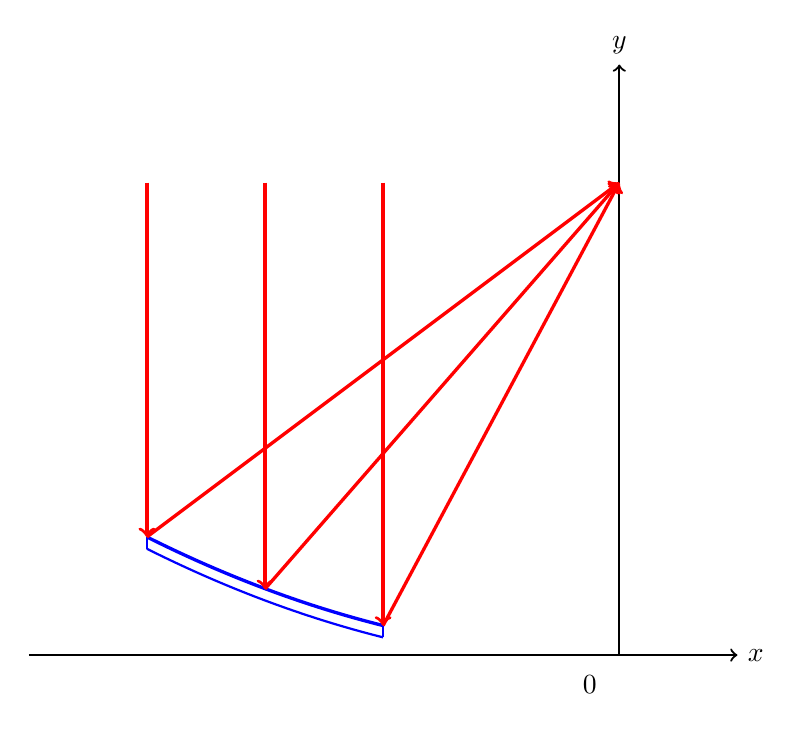
\begin{tikzpicture}[scale=1.5]
\def\f{4}
\def\xmin{-5} \def\xmax{1}
\def\ymin{0}  \def\ymax{5}
\def\fx{0} \def\fy{\f}
% draw axes
\draw (-.25,-.25) node[auto] {0};
\draw[->,thick] (\xmin,\ymin) -- (\xmax,\ymin) node[right] {$x$};
\draw[->,thick] (\ymin,\ymin) -- (\ymin,\ymax) node[above] {$y$};
% draw off-axis parabolic section
\draw[color=blue,very thick] plot [domain=-4:-2] (\x,{((\x)^2)/(4*\f)});
\draw[color=blue,thick] plot [domain=-4:-2] (\x,{((\x)^2)/(4*\f)-0.1});
\draw[-,color=blue,thick] (-4,{((-4)^2)/(4*\f)-0.1}) -- (-4,{((-4)^2)/(4*\f)});
\draw[-,color=blue,thick] (-2,{((-2)^2)/(4*\f)-0.1}) -- (-2,{((-2)^2)/(4*\f)});
% draw rays
\draw[->,color=red,very thick]  (-4,4) -- (-4,1); \draw[->,color=red,very thick]  (-4,1) -- (\fx,\fy);
\draw[->,color=red,very thick]  (-3,4) -- (-3,0.56); \draw[->,color=red,very thick]  (-3,0.56) -- (\fx,\fy);
\draw[->,color=red,very thick]  (-2,4) -- (-2,0.25); \draw[->,color=red,very thick]  (-2,0.25) -- (\fx,\fy);
\end{tikzpicture}
\caption{Nominal Raytrace}
\label{raytrace}
\end{figure}

 \subsection*{Objective}
 The objective of this analysis is to characterize the evolution of the focal point distribution when subjected to a random disturbance. This is accomplished by Monte Carlo Simulation (MCS) and an example based on user-defined values is presented in the results section. Furthermore, the functional dependence of the output distribution with respect to the input disturbance distribution is observed for a range user-defined values of the input distribution parameters and presented.
 
 % \subsection*{Assumptions}

% \begin{description}
	% \item[1)] The mirror section is an off-axis parabola.
	% \item[2)] All incoming plane waves focus to a single point.
	% \item[3)] The mirror surface is ideal and rigid.
	% \item[4)] The small angle approximation is valid for $\alpha$.
 % \end{description}